\documentclass[11pt]{article}
\usepackage[utf8]{inputenc}
\usepackage[T1]{fontenc}
\usepackage{lmodern}
\usepackage{geometry}
\usepackage{tikz}
\usetikzlibrary{arrows.meta,shapes.geometric}

\geometry{paperwidth=13cm,paperheight=6.9cm,margin=0cm}
\pagestyle{empty}
\setlength{\parindent}{0pt}

\definecolor{ctxFill}{RGB}{238,242,245}
\definecolor{ctxLine}{RGB}{155,168,179}
\definecolor{ctxText}{RGB}{38,52,67}
\definecolor{exFill}{RGB}{220,233,247}
\definecolor{exLine}{RGB}{23,54,93}
\definecolor{prFill}{RGB}{200,240,236}
\definecolor{prLine}{RGB}{8,127,140}
\definecolor{prText}{RGB}{6,79,87}
\definecolor{phFill}{RGB}{234,242,245}

\begin{document}
\noindent
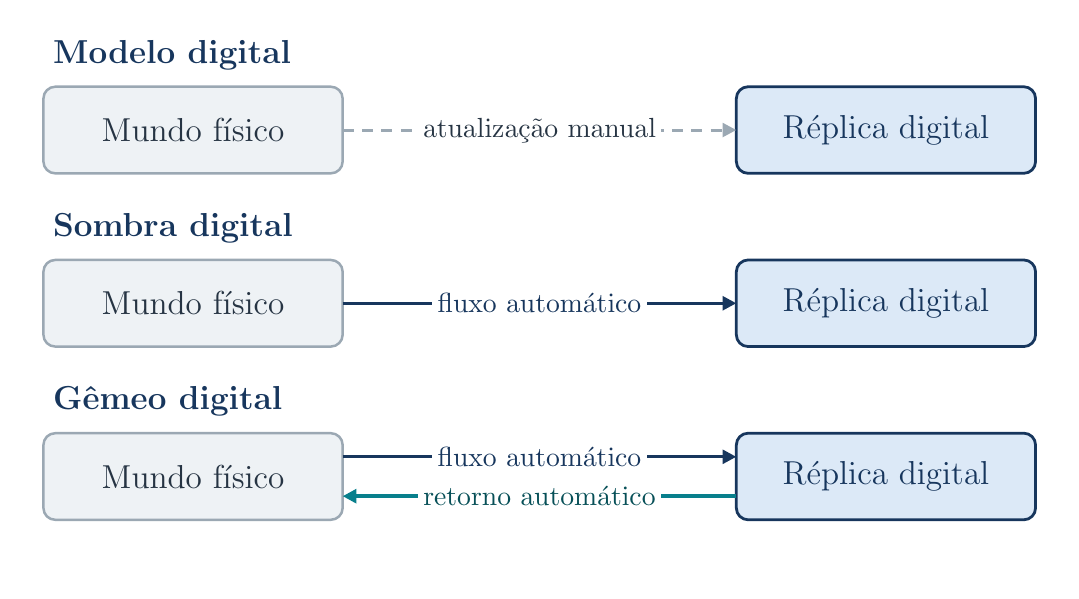
\begin{tikzpicture}[x=1cm,y=1cm,font=\small]
  \path[use as bounding box] (0,0) rectangle (13,6.9);
  \node[anchor=west,text=exLine] at (0.2,6.55) {\large\textbf{Modelo digital}};
  \draw[fill=ctxFill,draw=ctxLine,line width=0.9pt,rounded corners=0.15cm] (0.2,5.05) rectangle (4.0,6.1499999999999995);
  \node[text=ctxText] at (2.1,5.6) {\large Mundo físico};
  \draw[fill=exFill,draw=exLine,line width=1pt,rounded corners=0.15cm] (9.0,5.05) rectangle (12.8,6.1499999999999995);
  \node[text=exLine] at (10.9,5.6) {\large Réplica digital};
  \draw[draw=ctxLine,line width=1.1pt,dash pattern=on 4pt off 3pt,-{Triangle[length=5pt,width=5pt]}] (4.0,5.6) -- (9.0,5.6);
  \node[text=ctxText,fill=white,inner sep=2pt] at (6.5,5.6) {\normalsize atualização manual};
  \node[anchor=west,text=exLine] at (0.2,4.35) {\large\textbf{Sombra digital}};
  \draw[fill=ctxFill,draw=ctxLine,line width=0.9pt,rounded corners=0.15cm] (0.2,2.8499999999999996) rectangle (4.0,3.95);
  \node[text=ctxText] at (2.1,3.4) {\large Mundo físico};
  \draw[fill=exFill,draw=exLine,line width=1pt,rounded corners=0.15cm] (9.0,2.8499999999999996) rectangle (12.8,3.95);
  \node[text=exLine] at (10.9,3.4) {\large Réplica digital};
  \draw[draw=exLine,line width=1.2pt,-{Triangle[length=5pt,width=5pt]}] (4.0,3.4) -- (9.0,3.4);
  \node[text=exLine,fill=white,inner sep=2pt] at (6.5,3.4) {\normalsize fluxo automático};
  \node[anchor=west,text=exLine] at (0.2,2.15) {\large\textbf{Gêmeo digital}};
  \draw[fill=ctxFill,draw=ctxLine,line width=0.9pt,rounded corners=0.15cm] (0.2,0.6499999999999999) rectangle (4.0,1.75);
  \node[text=ctxText] at (2.1,1.2) {\large Mundo físico};
  \draw[fill=exFill,draw=exLine,line width=1pt,rounded corners=0.15cm] (9.0,0.6499999999999999) rectangle (12.8,1.75);
  \node[text=exLine] at (10.9,1.2) {\large Réplica digital};
  \draw[draw=exLine,line width=1.2pt,-{Triangle[length=5pt,width=5pt]}] (4.0,1.45) -- (9.0,1.45);
  \draw[draw=prLine,line width=1.4pt,-{Triangle[length=5pt,width=5pt]}] (9.0,0.95) -- (4.0,0.95);
  \node[text=exLine,fill=white,inner sep=2pt] at (6.5,1.45) {\normalsize fluxo automático};
  \node[text=prText,fill=white,inner sep=2pt] at (6.5,0.95) {\normalsize retorno automático};
\end{tikzpicture}
\end{document}
